%%%%%%%%%%%%%%%%%%%%%%%%%%%%%%%%%%%%%%%%%%%%%%%%%%%%%%%%%%%%%%%%%%%%%%%%
% Plantilla TFG/TFM
% Escuela Politécnica Superior de la Universidad de Alicante
% Realizado por: Jose Manuel Requena Plens
% Contacto: info@jmrplens.com / Telegram:@jmrplens
%%%%%%%%%%%%%%%%%%%%%%%%%%%%%%%%%%%%%%%%%%%%%%%%%%%%%%%%%%%%%%%%%%%%%%%%


% Ejemplo de páginas en horizontal y vertical

\chapter{Salidas de las implementaciones con GTKWave}
Aquí se muestra cómo incluir páginas en horizontal.

Esta página está en vertical\\
\clearpage % Nueva página

\begin{landscape} % Inicia modo horizontal
	

Esta página está en horizontal

\begin{figure}[ht]
	\centering
	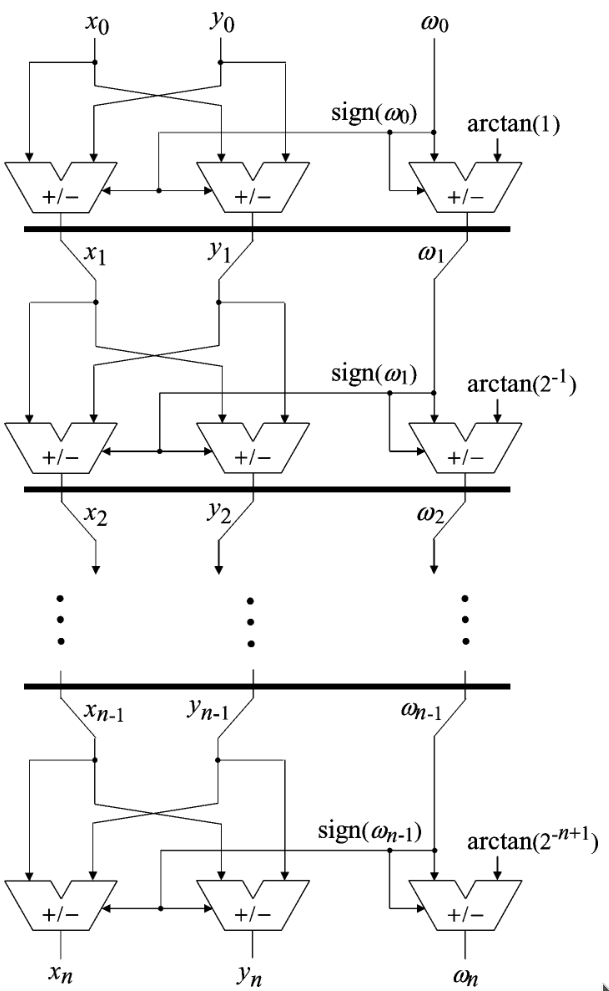
\includegraphics[width=0.50\textwidth]{archivos/CORDIC/2009-CORDIC_pipelined.png}
	\caption{\gls{cordic} convencional con \textit{pipelining}}
	\label{graf:2009-CORDIC_pipelined}
\end{figure}


\clearpage % Nueva página

Esta página también está en horizontal\\

\end{landscape} % Finaliza modo horizontal
\clearpage % Nueva página


Esta página está de nuevo en vertical\\